\renewcommand*{\figurename}{Dato}
\section*{Retoques finales al inicio}
\begin{frame}
    El motor estaría de una forma muy resumida y simple, presentado acá, faltaría mencionar algunos extras que agregué.
    \begin{itemize}
        \item Tiempo de búsqueda y cantidad de resultados encontradas
        \begin{figure}
            \centering
            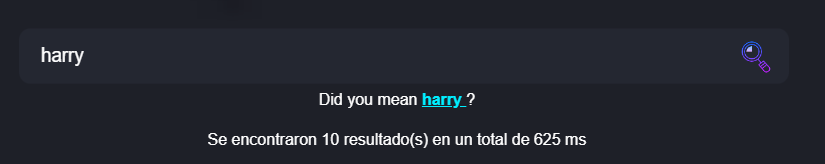
\includegraphics[width=260px]{Assets/time_results.png}
        \end{figure}
        \item Arriba a la derecha se puede ver:
        \begin{figure}
            
\includegraphics[height=25px, width=25px]{Assets/mode.png}
            \caption{Una utilidad para cambiar el modo visual de la región gráfica.}
        \end{figure}
    \end{itemize}
\end{frame}

\section*{Finally the end}
\begin{frame}
    \begin{figure}
        \centering
        
\includegraphics[width=150px]{Assets/the_end.png}
    \end{figure}
\end{frame}